% =============================================================================
% Chapter 1: Introduction
% NexaLearn Graduation Project — Cairo University, Faculty of Engineering
% =============================================================================

\chapter{Introduction}
\label{ch:introduction}

This chapter introduces \textbf{NexaLearn}, a production-oriented e-learning backend platform developed as the graduation project of the Department of Computer Engineering at Cairo University, Faculty of Engineering. NexaLearn is an AI-augmented, commerce-enabled learning platform backend implemented as a NestJS modular monolith in TypeScript, backed by PostgreSQL, Redis, and a suite of managed external services including Stripe, Mux, and AWS S3. The system is organised into sixteen domain bounded contexts and four infrastructure modules, grouped into three high-level capability areas: the \emph{Learning Core} (authentication, courses, enrollment, media, progress, assessment, certificates), \emph{Engagement \& Commerce} (discussion, reviews, streaks, notifications, payments, search), and \emph{Platform \& Operations} (instructor analytics, administration, audit logging, event infrastructure, AI pipeline orchestration, and shared data access).

The purpose of this chapter is fivefold. First, it establishes \textit{why} such a platform is needed in the current e-learning market and why existing alternatives---commercial SaaS products, legacy open-source LMS platforms, and generic web boilerplates---fail to provide a cohesive reference for modern backend engineering. Second, it defines the \textit{problems} that NexaLearn explicitly sets out to solve, including unreliable asynchronous integrations, architectural erosion across many bounded contexts, financial and AI callback integrity, and privacy-preserving analytics. Third, it states measurable \textit{objectives} that govern design and implementation decisions throughout the project. Fourth, it enumerates the \textit{outcomes}---REST APIs, database schema, deployment stack, OpenAPI documentation, integration tests, and architecture records---that constitute the deliverable artefacts. Fifth, it explains how the remainder of this report is organised so that evaluators and future readers can navigate from market context through literature, detailed design, verification, and conclusions.

NexaLearn is conceived not merely as a collection of REST endpoints, but as a \textit{reference architecture}: a codebase and accompanying documentation that demonstrate how Domain-Driven Design (DDD), Clean Architecture, CQRS-lite read/write separation, event-driven integration via a transactional outbox, and production reliability patterns (idempotency keys, optimistic concurrency control, HMAC-verified webhooks, refresh-token rotation) can be applied to the full vertical stack of an online learning marketplace. A student enrolling in a paid course, watching transcoded video lessons, attempting AI-generated quizzes, participating in moderated discussions, earning a certificate, and leaving a review triggers a coordinated chain of domain events spanning more than half of the bounded contexts in the system. Chapter~1 frames the engineering ambition required to implement such workflows correctly, setting the stage for the technical depth presented in subsequent chapters.

% =============================================================================
% Section 1.1: Motivation and Justification
% =============================================================================

\section{Motivation and Justification}
\label{sec:motivation}

\subsection{The Post-COVID E-Learning Market}
\label{subsec:post-covid-market}

The global e-learning industry has undergone a structural and likely permanent transformation since the COVID-19 pandemic forced universities, training providers, and enterprises to deliver instruction remotely at unprecedented scale. What was previously treated as a supplementary channel---useful for corporate compliance modules or distance-learning electives---has become a primary delivery mechanism for degree programmes, professional certification, and independent creator economies. Industry analyses value the global e-learning market at approximately \$250--400~billion in the mid-2020s, with compound annual growth rates consistently projected in the double digits through the end of the decade. Growth drivers include corporate upskilling mandates, higher-education digitisation, mobile-first learners in emerging markets, and the proliferation of creator-led course businesses.

Leading commercial platforms illustrate the scale that modern backends must support. \textbf{Udemy} reports tens of millions of registered learners and hundreds of millions of course enrolments cumulatively; peak traffic during promotional events stresses payment, entitlement, and content-delivery subsystems simultaneously. \textbf{Coursera} partners with universities worldwide and must reconcile academic calendars, verified credentials, and enterprise B2B contracts within shared infrastructure. \textbf{LinkedIn Learning}, \textbf{edX}, and regional platforms such as \textbf{Udacity} and \textbf{Pluralsight} similarly combine video libraries, assessments, progress tracking, and monetisation in unified user experiences. Although NexaLearn is scoped as a graduation project rather than a hyperscale production deployment, it is deliberately engineered against the \textit{functional} and \textit{architectural} expectations these platforms establish: stateless horizontally scalable API tiers, durable workflow orchestration, secure payment settlement, entitlement-aware media delivery, and analytics that inform instructor and operator decisions.

The post-COVID era also normalised hybrid instructional models in which asynchronous video modules coexist with synchronous sessions, formative AI-generated quizzes supplement summative exams, and discussion forums extend classroom dialogue. Backend systems must therefore support not only CRUD operations on course catalogues, but long-running asynchronous pipelines (transcoding, transcription, question generation), fine-grained authorisation (instructor, student, admin, teaching assistant roles), and cross-module eventual consistency without sacrificing user-visible correctness.

\subsection{Fragmentation of Existing Open-Source and Template Solutions}
\label{subsec:fragmentation}

Despite market maturity, the software engineering community lacks a cohesive, open, and pedagogically transparent backend that unifies the full breadth of e-learning concerns within a single architecturally disciplined codebase. The gap manifests in three distinct categories of alternative, each insufficient as a holistic reference.

\textbf{Commercial closed platforms.} Udemy, Coursera, Teachable, Thinkific, and Kajabi deliver polished end-user experiences but expose only narrow public APIs. Internal service boundaries, saga implementations, event schemas, and consistency models remain trade secrets. Independent engineering teams cannot inspect how enrollment activation is coupled to payment webhooks, how video DRM integrates with progress checkpoints, or how AI-generated assessments are validated before publication. Vendor lock-in and revenue-sharing models further discourage universities and startups seeking data sovereignty.

\textbf{Legacy open-source LMS platforms.} Moodle, Sakai, and Canvas (open-core) evolved over decades as plugin-oriented PHP or Java monoliths. They prioritise feature breadth---forums, gradebooks, SCORM players, attendance plugins---over modular domain clarity. Cross-plugin coupling, shared global state, and inconsistent API layers make it difficult to extract modern patterns such as bounded contexts, transactional outboxes, or typed domain events. Moodle's architecture, while battle-tested at institutional scale, reflects design decisions from an era before widespread REST microservices, TypeScript type safety, and cloud-native video pipelines.

\textbf{Specialised micro-templates and generic boilerplates.} The NestJS ecosystem offers numerous starter repositories providing JWT authentication, Prisma CRUD, and Docker Compose scaffolding. Separate commercial services address individual verticals: Stripe for payments, Mux or Cloudflare Stream for video, Algolia for search, SendGrid for email. None of these templates demonstrate how fifteen or more bounded contexts should collaborate under shared transactional guarantees, nor do they implement e-learning-specific state machines (pending enrollment awaiting payment, video asset awaiting transcoding, quiz attempt awaiting async grading). Developers assembling these pieces ad hoc frequently produce systems that \textit{appear} functional in demos but fail under duplicate webhook delivery, concurrent course edits, or partial pipeline failures.

Table~\ref{tab:platform-comparison-intro} summarises the principal limitation motivating NexaLearn: no widely available open reference spans authentication, structured course aggregates, payment-backed enrollment, Mux-integrated media, Whisper/LLM AI pipelines, assessment, social learning, certificates, search, streaks, notifications, and instructor analytics within one DDD-governed NestJS codebase.

\begin{table}[H]
  \centering
  \caption{High-Level Comparison of Platform Categories Relevant to NexaLearn Motivation}
  \label{tab:platform-comparison-intro}
  \small
  \begin{tabular}{@{}p{2.8cm} p{3.2cm} p{3.5cm} p{3.8cm}@{}}
    \toprule
    \textbf{Category} & \textbf{Representative Examples} & \textbf{Primary Strengths} & \textbf{Gap NexaLearn Addresses} \\
    \midrule
    Commercial SaaS &
    Udemy, Coursera, Teachable &
    Polished UX, scale, content marketplace &
    No source access; opaque architecture; vendor lock-in \\
    \addlinespace
    Legacy OSS LMS &
    Moodle, Open edX, Sakai &
    Institutional adoption; rich plugin ecosystems &
    Monolithic plugin sprawl; dated stacks; weak DDD \\
    \addlinespace
    Generic NestJS starters &
    Community boilerplates &
    Fast bootstrap; JWT + ORM patterns &
    No e-learning domain; no outbox; no Stripe/Mux/AI \\
    \addlinespace
    Vertical SaaS APIs &
    Stripe, Mux, OpenAI &
    Best-in-class single concern &
    No unified domain model or cross-context reliability \\
    \bottomrule
  \end{tabular}
\end{table}

\subsection{Architectural Challenges Facing E-Learning Backend Developers}
\label{subsec:architectural-challenges}

Developers who attempt to build e-learning platforms from scratch encounter recurring architectural challenges that introductory web development curricula rarely address. These challenges form the technical core of NexaLearn's motivation.

\textbf{Cross-bounded-context workflow orchestration.} A representative student journey traverses Search (discovery), Enrollment (intent), Payments (settlement), Courses/Media (consumption), Progress (checkpointing), Assessment (validation), Certificates (credential), Reviews (feedback), Notifications (engagement), and Streak (retention). Each step is owned by a distinct module with its own aggregates and invariants. Naive implementations invoke synchronous service calls across module boundaries, creating availability cascades and tight coupling. Event-driven designs alleviate synchronous coupling but introduce delivery semantics questions: what happens if the notification dispatcher fails after enrollment activates?

\textbf{Eventual consistency and external callbacks.} Video platforms emit webhooks when uploads complete or renditions become playable; Stripe notifies applications of \texttt{payment\_intent.succeeded} and \texttt{charge.refunded}; AI workers callback with transcription segments or generated question banks minutes to hours later. Network retries cause duplicate deliveries; maintenance windows cause delayed out-of-order arrivals. Without idempotent handlers backed by persistent idempotency keys or outbox deduplication, systems exhibit double enrollment activation, orphaned Mux assets detached from lessons, or students charged without course access---failures that erode trust and create support burden.

\textbf{Concurrency and aggregate integrity.} Instructors reorder lessons while students mark progress; admins publish course revisions while enrollment counts feed analytics dashboards. Lost updates on course structures, duplicate quiz attempts, and race conditions on seat-limited offerings require optimistic or pessimistic concurrency strategies encoded at the domain layer, not patched ad hoc in controllers.

\textbf{Security and compliance surface area.} Authentication must resist credential stuffing (rate limiting), token theft (refresh rotation with reuse detection), and privilege escalation (RBAC with instructor-scoped analytics). Payment endpoints must verify webhook signatures. AI pipeline callbacks must authenticate via HMAC to prevent forged quiz injection. Audit trails must record administrative actions without storing secrets or raw payment instrument data.

\subsection{The AI Imperative in Modern E-Learning}
\label{subsec:ai-imperative}

A further motivation distinct from pre-2020 LMS development is the rapid integration of artificial intelligence into educational workflows. Learners expect searchable transcripts of video lectures; instructors seek automated generation of formative multiple-choice and short-answer questions aligned with lesson content; platform operators explore async grading assistance for open-ended responses to scale human review. These capabilities are not cosmetic feature flags---they imply dedicated pipeline orchestration, job state tracking, cost-aware retry policies, content moderation boundaries, and privacy controls over copyrighted or personally identifiable material submitted to third-party models.

Speech-to-text models such as \textbf{OpenAI Whisper} produce transcripts that feed retrieval and accessibility features. Large language models (LLMs) synthesise question banks when prompted with transcript segments and instructor constraints (difficulty, count, question types). Such pipelines are inherently \textit{asynchronous} and \textit{non-deterministic}: failures, partial results, and model revisions must be handled gracefully without corrupting published assessment entities. Treating AI as a bolt-on script rather than a first-class \textbf{AI Pipeline bounded context} leads to duplicated callback endpoints, inconsistent correlation identifiers, and security gaps when unsigned webhook payloads mutate production quiz data.

NexaLearn addresses this imperative by modelling AI jobs as domain entities with explicit lifecycle states (\texttt{queued}, \texttt{processing}, \texttt{completed}, \texttt{failed}), securing service-to-service calls with HMAC signatures, and applying idempotent callback processing so retried pipeline notifications never duplicate questions or overwrite instructor edits.

\begin{figure}[H]
  \centering
  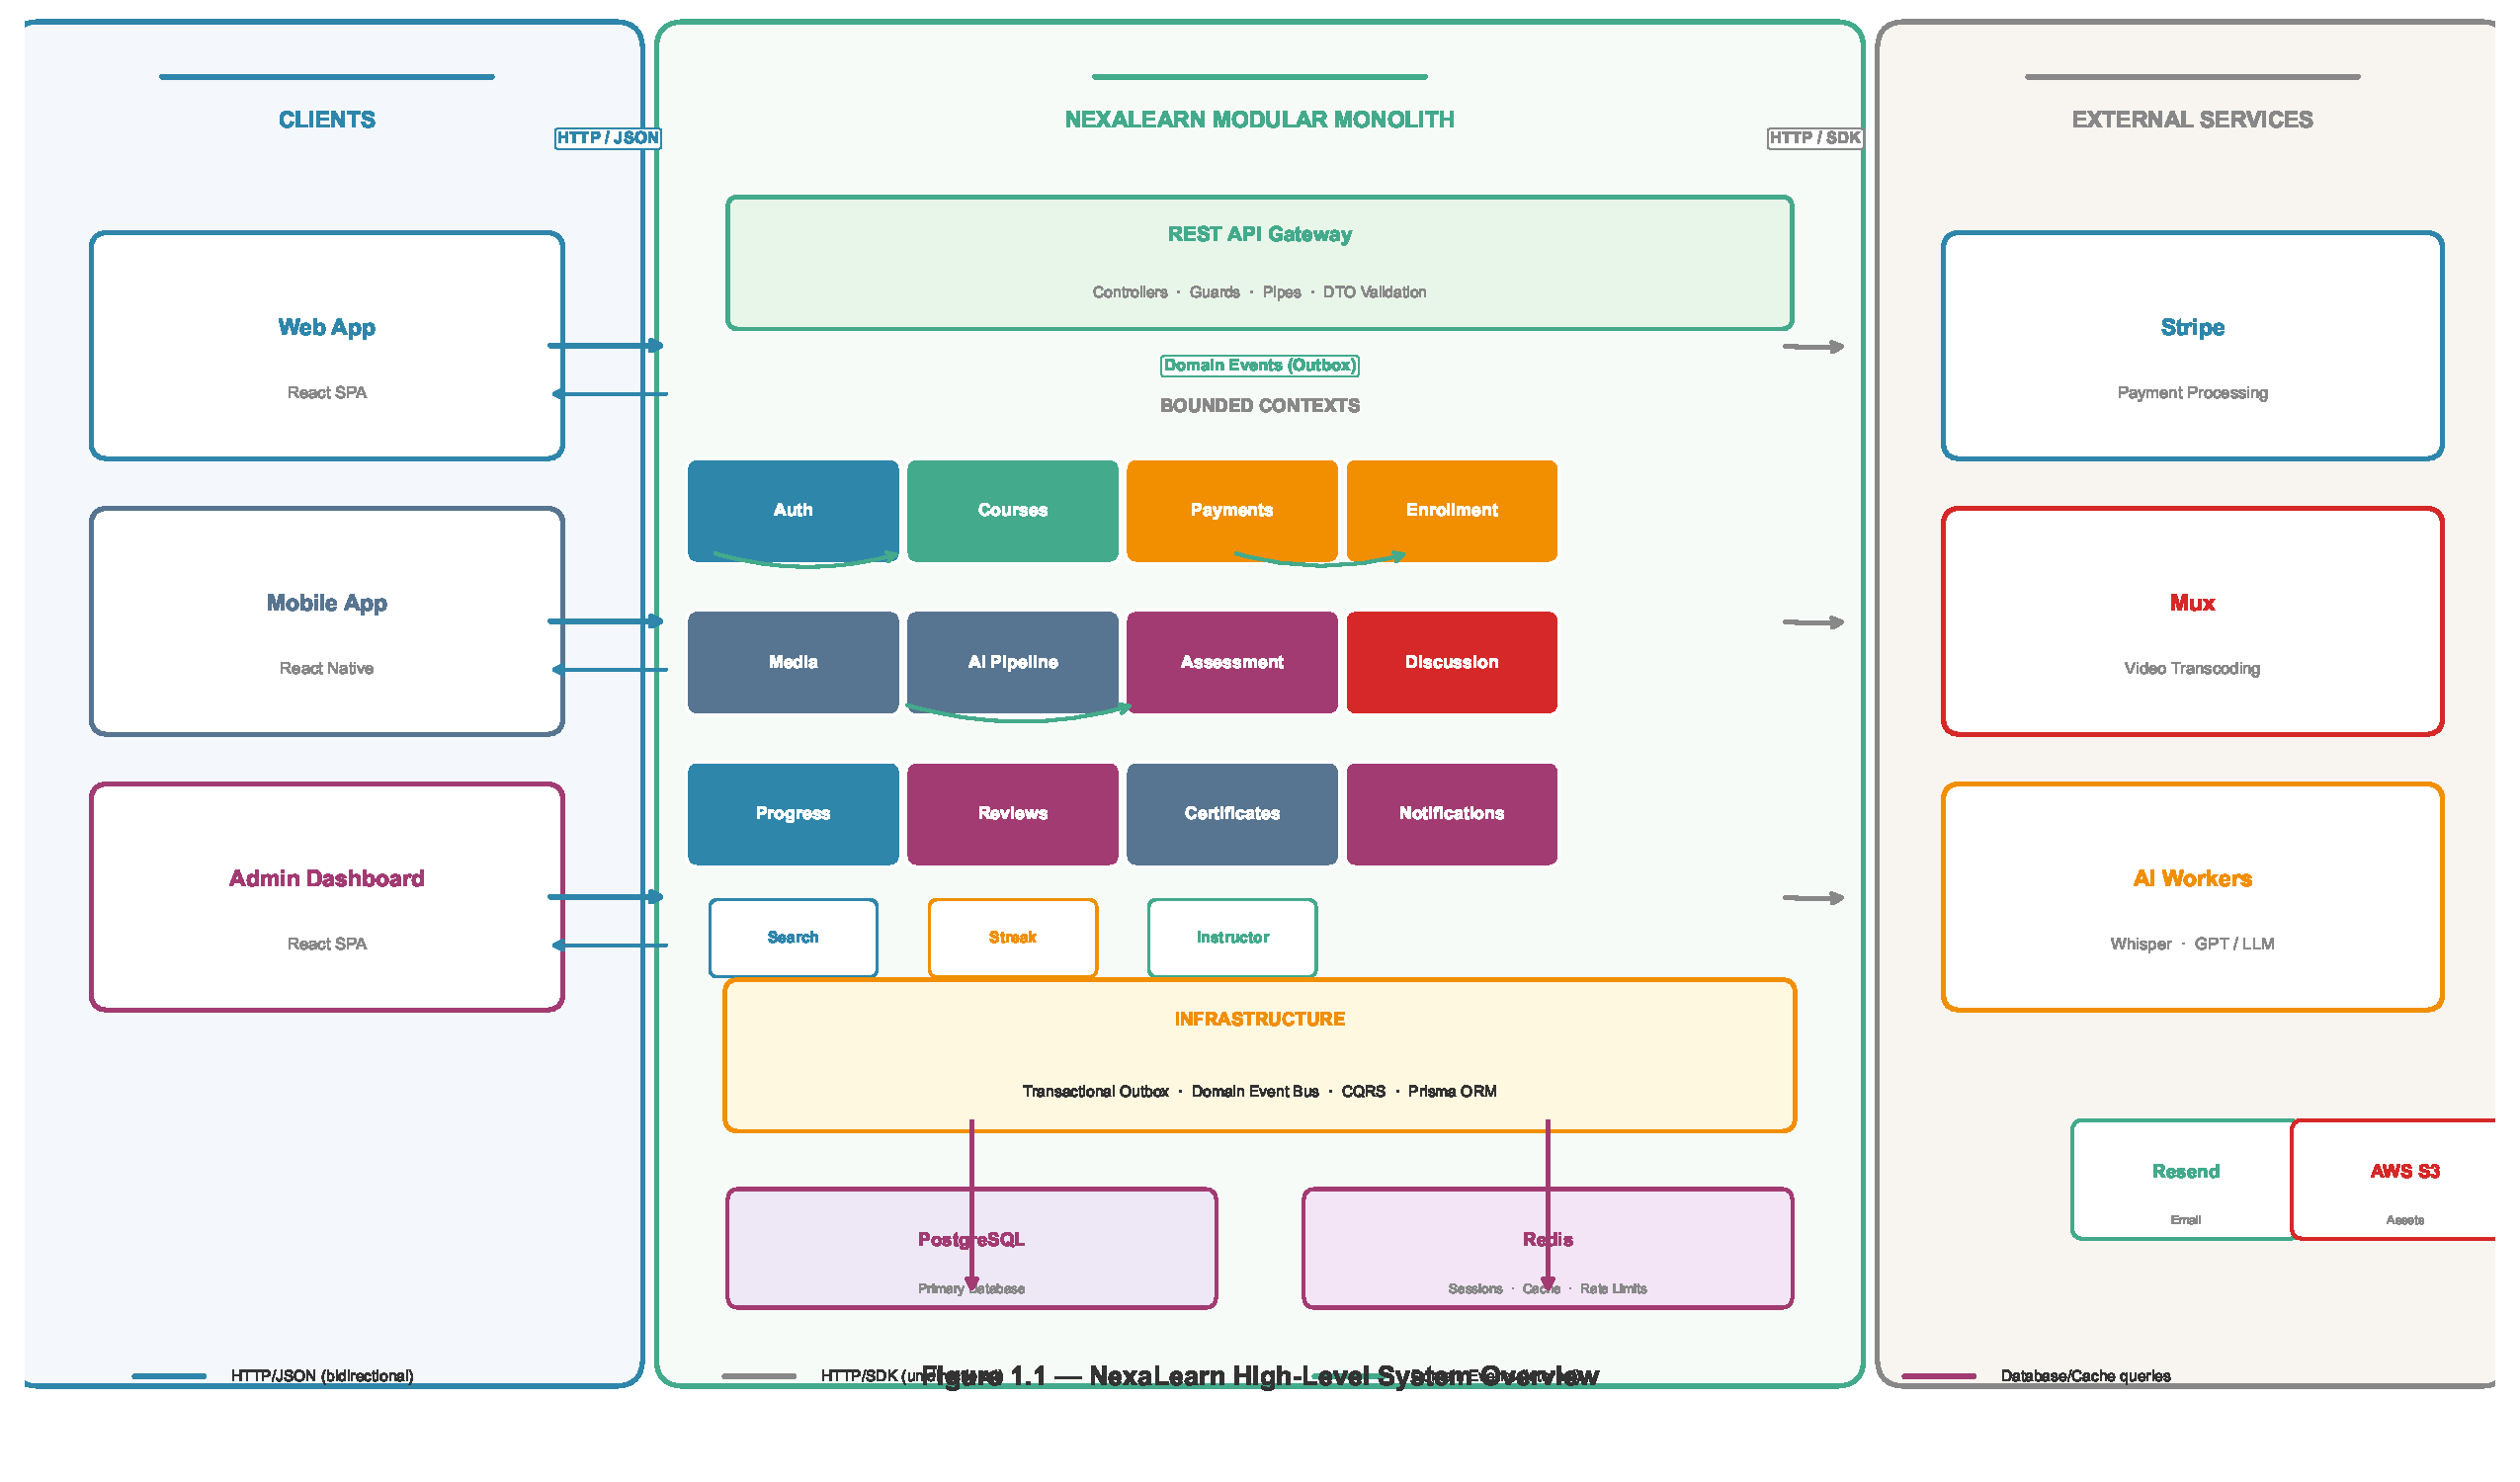
\includegraphics[width=\textwidth]{images/system_overview.pdf}
  \caption{NexaLearn High-Level System Overview}
  \label{fig:system-overview}
\end{figure}

Figure~\ref{fig:system-overview} illustrates NexaLearn's placement within the broader ecosystem: client applications (web, mobile, admin dashboards) consume a REST API exposed by a modular monolith; internal modules communicate via domain events persisted to a transactional outbox; external integrations include Stripe (payments), Mux (video), AWS S3 (supplementary assets), Resend or equivalent (transactional email), Redis (sessions, cache, rate limits), and external AI workers (Whisper transcription, LLM question generation). The diagram reflects a deliberate \textit{modular monolith} stance---operational simplicity with internal seams ready for future extraction if scale demands.

\subsection{Justification of the NexaLearn Approach}
\label{subsec:justification}

The justification for undertaking NexaLearn as a graduation project rests on four pillars aligned with both academic evaluation criteria and industry practice.

\textbf{Reference implementation gap.} No widely cited open codebase demonstrates end-to-end e-learning backend composition with DDD, Clean Architecture, transactional outbox, Stripe/Mux/AI integrations, and Testcontainers-backed integration tests in TypeScript. NexaLearn fills this gap for students, instructors evaluating the project, and future teams seeking a reproducible starting point.

\textbf{Production-grade reliability as a learning objective.} Computer Engineering graduates must understand patterns that distinguish demo-quality software from operable systems: idempotency, exactly-once side effects, webhook signature verification, optimistic locking, and structured audit logging. NexaLearn embeds these patterns in working code with tests, not merely in slides.

\textbf{Modular monolith pragmatism.} Microservice decomposition introduces distributed tracing, service mesh, and cross-service transaction complexity disproportionate to a graduation project timeline. A well-structured modular monolith delivers clear module boundaries and event-driven decoupling while remaining deployable via Docker Compose---satisfying the faculty requirement that interested readers could replicate the system without a Kubernetes cluster.

\textbf{Capstone coherence for Cairo University.} The project integrates database design, API engineering, security, cloud service integration, AI pipeline orchestration, and software architecture---competencies expected of Computer Engineering graduates. The resulting artefact is defensible in viva examination, extensible by subsequent cohorts, and portfolio-worthy for industry recruitment.

In summary, NexaLearn is motivated by market scale, architectural fragmentation in existing alternatives, the non-trivial reliability demands of async e-learning workflows, and the emerging necessity of AI-augmented content pipelines---and justified as a rigorous, open reference that future engineers can study, deploy, and improve.

% =============================================================================
% Section 1.2 (Part A): Problem Definition
% =============================================================================

\section{Project Objectives and Problem Definition}
\label{sec:problem-objectives}

\subsection{Problem Definition}
\label{subsec:problem-definition}

The central research and engineering problem addressed by this graduation project is stated formally below.

\begin{quote}
\textit{Given a multi-stakeholder e-learning platform serving concurrent students, instructors, and administrators, how can a team design and implement a complete, open, production-ready backend that coordinates authentication, structured course management, video media lifecycles, AI-generated educational content, financial transactions, learner engagement features, and privacy-preserving instructor analytics---while preserving domain clarity across fifteen or more bounded contexts, guaranteeing reliable asynchronous integration with external providers, and maintaining ACID consistency for business-critical state transitions?}
\end{quote}

This overarching problem decomposes into six interrelated sub-problems, each corresponding to observable failure modes in real-world e-learning systems and motivating explicit architectural responses in NexaLearn.

\subsubsection{Lack of Complete Vertical Coverage in Open Backends}
\label{subsubsec:vertical-coverage}

Most publicly available backend templates and partial LMS implementations excel at isolated vertical slices---user registration with JSON Web Tokens (JWT), file upload to object storage, or a basic quiz engine---but fail to implement the \textit{full lifecycle} of a commercial e-learning product within one cohesive domain model. Consider a single paid enrollment: the system must validate course availability and pricing, create a pending enrollment record, initiate a Stripe PaymentIntent, await a signed webhook confirming payment, atomically activate enrollment, initialise progress projections for all lessons, grant Mux playback entitlements, enqueue welcome notifications, update search-facing enrollment statistics, and record audit events---all while remaining resilient to duplicate client retries and partial failures.

When these concerns are implemented as an undifferentiated ``services'' layer without bounded contexts, implicit coupling emerges rapidly. Payment services begin mutating enrollment tables directly; progress services bypass assessment prerequisites; search reads denormalised columns that drift when outbox processors lag. The sub-problem is therefore not merely absent features, but the absence of a \textit{ubiquitous language} and \textit{context map} assigning ownership, invariants, and published integration contracts to each concern. NexaLearn responds by defining sixteen domain modules---Auth, Courses, Enrollment, Payments, Media, AI Pipeline, Assessment, Discussion, Progress, Reviews, Certificates, Search, Streak, Notifications, Instructor, and Admin---plus infrastructure modules for Prisma, Events, and Audit.

\subsubsection{Unreliable Asynchronous Event Processing}
\label{subsubsec:async-events}

E-learning backends are inherently event-heavy. Representative external event sources include:
\begin{itemize}
  \item \textbf{Mux webhooks} --- \texttt{video.asset.ready}, upload cancellation, encoding errors;
  \item \textbf{Stripe webhooks} --- \texttt{payment\_intent.succeeded}, \texttt{payment\_intent.payment\_failed}, \texttt{charge.refunded}, \texttt{checkout.session.completed};
  \item \textbf{AI pipeline callbacks} --- transcription completion, generated question payloads, grading results for short-answer items;
  \item \textbf{Internal domain events} --- \texttt{EnrollmentActivated}, \texttt{LessonCompleted}, \texttt{QuizAttemptSubmitted}, \texttt{CertificateIssued}.
\end{itemize}

Network partitions, at-least-once delivery guarantees from cloud providers, and application restarts during consumer processing make duplicate and out-of-order delivery \textit{normal} rather than exceptional. Naive ``publish to message broker after commit'' approaches suffer the dual-write problem: database commits succeed while message publication fails, or vice versa. NexaLearn must achieve \textit{at-least-once transport with exactly-once side effects} without two-phase commit across heterogeneous systems. The chosen pattern---\textbf{transactional outbox} with row-level locking via \texttt{SELECT FOR UPDATE SKIP LOCKED}---persists events in the same PostgreSQL transaction as domain mutations, then processes them idempotently through dedicated handlers that update projections, dispatch notifications, and trigger downstream workflows.

\subsubsection{Architectural Erosion Across Many Bounded Contexts}
\label{subsubsec:bounded-context-erosion}

Domain-Driven Design recommends decomposing complex domains into bounded contexts with explicit upstream/downstream relationships, anti-corruption layers for external models, and context maps documenting integration styles (shared kernel, customer-supplier, conformist, open-host service). In practice, naively creating fifteen or more NestJS modules without enforced dependency rules yields circular imports, anaemic entities that mirror database rows without behaviour, and repository leakage where controllers query foreign context tables directly.

The sub-problem is organisational and technical: maintain Clean Architecture layering (domain innermost; application use cases; infrastructure adapters outermost) across twenty NestJS modules while preserving developer velocity. Dependency constraints require that Courses never import Payments repositories; Discussion never writes Progress tables; Instructor analytics reads through authorised query services rather than ad hoc joins. Without discipline, the modular monolith collapses into the monolithic ``ball of mud'' it was intended to prevent.

\subsubsection{Exactly-Once Semantics for Financial and AI Integrations}
\label{subsubsec:financial-ai-integrity}

Monetary transactions and machine-generated assessments carry elevated correctness, regulatory, and reputational requirements. Failure modes include:
\begin{itemize}
  \item duplicate Stripe webhook $\rightarrow$ double enrollment activation or duplicate revenue recognition;
  \item lost refund webhook $\rightarrow$ student retains access after chargeback;
  \item replayed AI callback $\rightarrow$ duplicate quiz questions or overwritten instructor edits;
  \item forged unsigned callback $\rightarrow$ injection of malicious assessment content.
\end{itemize}

Conversely, legitimately retried webhooks after transient 503 responses must succeed without manual operations intervention. NexaLearn must implement \textit{idempotent, auditable integration endpoints} with Stripe signature verification, HMAC-authenticated AI pipeline callbacks, structured correlation identifiers (\texttt{enrollmentId}, \texttt{pipelineJobId}, \texttt{idempotencyKey}), and persistent deduplication stores recording processed event fingerprints.

\subsubsection{Privacy-Preserving Instructor Analytics}
\label{subsubsec:privacy-analytics}

Instructors require aggregated insights---module completion funnels, median quiz scores, revenue by course offering, streak participation rates, discussion engagement---to improve content and pricing decisions. Platform administrators require security dashboards (failed login spikes, token reuse alerts). However, indiscriminate SQL joins across \texttt{User}, \texttt{Enrollment}, \texttt{LessonProgress}, and \texttt{Payment} tables risk exposing personally identifiable information (PII), enabling re-identification in small cohorts, or allowing Instructor~A to infer performance data for courses they do not own.

The sub-problem is to deliver \textit{actionable analytics through dedicated application services} that enforce role-based access control (RBAC), aggregate at safe granularities, parameterise queries by \texttt{instructorId} derived from authenticated identity rather than client-supplied filters, and never return row-level student identifiers in instructor-facing revenue or engagement exports unless explicitly authorised for institutional admin roles.

\subsubsection{Stakeholder Expectations and Non-Functional Constraints}
\label{subsubsec:stakeholder-nfr}

Beyond functional gaps, the problem includes satisfying diverse stakeholder non-functional requirements simultaneously. Table~\ref{tab:stakeholder-requirements} maps primary stakeholders to expectations that constrain architecture.

\begin{table}[H]
  \centering
  \caption{Stakeholder Groups and Their Architectural Expectations in NexaLearn}
  \label{tab:stakeholder-requirements}
  \small
  \begin{tabular}{@{}p{2.6cm} p{4.2cm} p{6.8cm}@{}}
    \toprule
    \textbf{Stakeholder} & \textbf{Primary Concerns} & \textbf{Architectural Implications} \\
    \midrule
    Students &
    Fair access after payment; reliable video playback; accurate grades &
    Idempotent enrollment activation; signed Mux URLs; atomic quiz finalisation \\
    \addlinespace
    Instructors &
    Content control; AI assistance; performance insights &
    OCC on course aggregates; AI job tracking; scoped analytics queries \\
    \addlinespace
    Platform admins &
    Security; auditability; moderation &
    RBAC; Audit module; admin dashboards; rate limiting \\
    \addlinespace
    Developers &
    Maintainability; testability; clear boundaries &
    DDD modules; outbox tests; OpenAPI docs; Docker Compose \\
    \addlinespace
    Evaluators &
    Reproducibility; self-contained documentation &
    Migrations; integration tests; this report \\
    \bottomrule
  \end{tabular}
\end{table}

\begin{figure}[H]
  \centering
  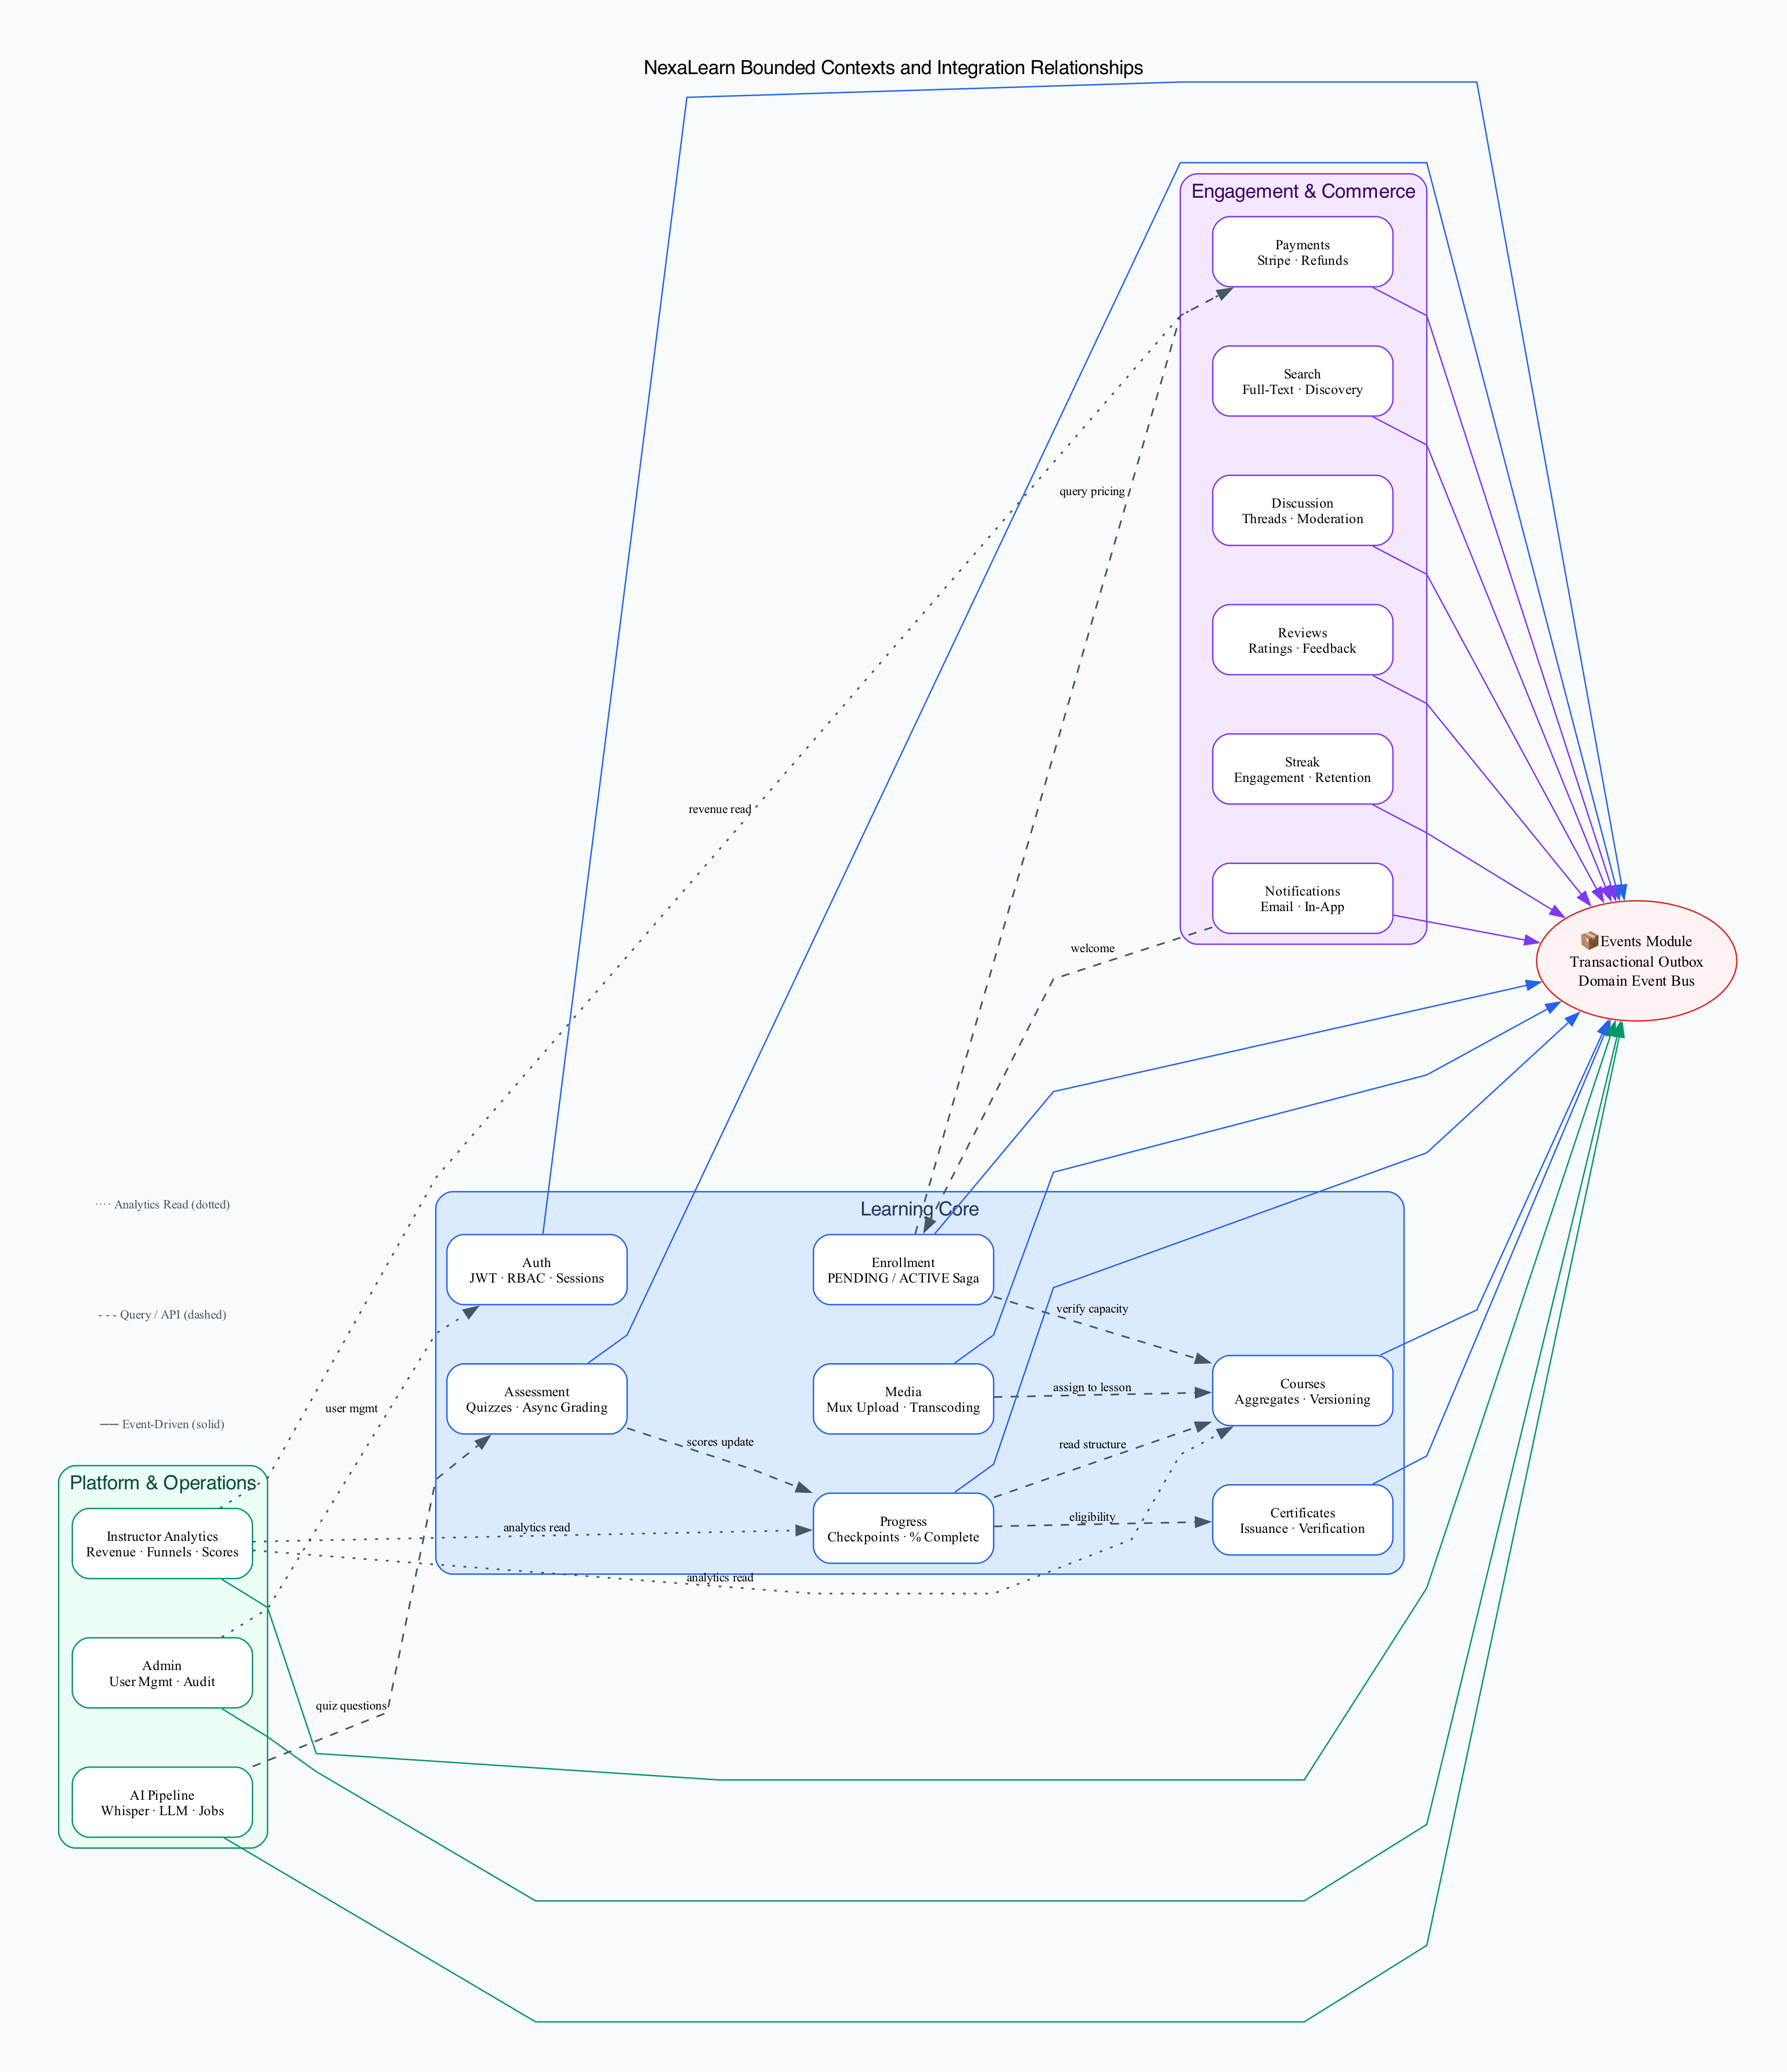
\includegraphics[width=0.88\textwidth]{images/bounded_contexts.png}
  \caption{NexaLearn Bounded Contexts and Integration Relationships}
  \label{fig:bounded-contexts}
\end{figure}

Figure~\ref{fig:bounded-contexts} visualises the sixteen domain bounded contexts and their primary event-driven (solid) and query/API-driven (dashed) relationships. Three high-level groupings---Learning Core, Engagement \& Commerce, Platform \& Operations---provide cognitive structure without implying separate deployable microservices. The Events module and transactional outbox sit centrally because nearly every context publishes or consumes domain integration events.

Collectively, these sub-problems define a problem space where superficial feature accumulation fails; only explicit domain modelling, reliability patterns, and layered architecture can produce a backend that remains correct under concurrency, trustworthy under duplicate webhooks, and comprehensible to engineers who inherit the codebase after graduation.

% =============================================================================
% Section 1.2 (Part B): Project Objectives
% =============================================================================

\subsection{Project Objectives}
\label{subsec:project-objectives}

In direct response to the problems defined in Section~\ref{subsec:problem-definition}, NexaLearn pursues eight primary objectives. Each objective is stated as an implementable goal, accompanied by success criteria verifiable through code inspection, automated tests, or API demonstration. Objectives map to bounded contexts and cross-cutting mechanisms described in detail in Chapter~4.

\begin{enumerate}
  \item \textbf{Implement a secure, JWT-based authentication system with refresh token rotation and Redis session management.}

  The Auth bounded context shall deliver complete identity lifecycle management: user signup with email verification tokens, password reset via time-limited secrets, login issuing short-lived access JWTs and opaque refresh tokens, logout invalidating refresh token families, and token refresh with \textit{rotation}---each refresh retires the previous token and detects reuse indicative of theft.

  \textit{Success criteria:} Argon2 password hashing; refresh tokens stored as hashes; Redis-backed session metadata and optional blocklists; global rate limiting via \texttt{@nestjs/throttler} with Redis storage; RBAC roles (\texttt{STUDENT}, \texttt{INSTRUCTOR}, \texttt{ADMIN}) enforced by guards on protected routes; integration tests covering login, refresh rotation, and reuse detection.

  \item \textbf{Build a course management system with DDD aggregates supporting modules, lessons, and optimistic concurrency.}

  The Courses context shall model \texttt{Course} as an aggregate root containing ordered \texttt{Module} entities, each containing ordered \texttt{Lesson} entities with publication states (\texttt{DRAFT}, \texttt{PUBLISHED}, \texttt{ARCHIVED}). Use cases include create/update course metadata, add/reorder modules and lessons, attach prerequisites, and publish revisions visible to enrolled students.

  \textit{Success criteria:} Domain invariants enforced in entities (e.g., cannot publish empty course); optimistic concurrency via \texttt{version} column-throws on conflict; domain events (\texttt{CoursePublished}, \texttt{LessonAdded}) emitted to outbox; instructor ownership validated on every mutation; no direct Prisma calls from controllers.

  \item \textbf{Integrate the Mux video platform for upload, transcoding, and signed playback URLs.}

  The Media context shall orchestrate Mux direct uploads, persist \texttt{VideoAsset} entities tracking provider identifiers and status (\texttt{WAITING}, \texttt{PROCESSING}, \texttt{READY}, \texttt{ERROR}), process signed Mux webhooks idempotently, associate ready assets with lessons, and issue signed playback tokens restricted to enrolled students.

  \textit{Success criteria:} Webhook signature verification; idempotent handler keyed by Mux event identifier; playback authorisation integrated with Enrollment/Progress guards; instructor dashboard listing assets with error diagnostics; integration test simulating webhook delivery.

  \item \textbf{Build an AI pipeline integration for automatic quiz generation and transcript creation using Whisper.}

  The AI Pipeline context shall accept instructor-initiated jobs bound to lesson video assets, submit HMAC-signed requests to external transcription (Whisper) and LLM question-generation workers, track job status transitions, and process asynchronous callbacks idempotently to create or update Assessment entities (transcripts, draft questions) without duplicating content on retries.

  \textit{Success criteria:} \texttt{PipelineJob} entity with lifecycle states; correlation IDs linking jobs to lessons and instructors; callback authentication; instructor review gate before student-visible quiz publication; failure records with retry policy.

  \item \textbf{Implement a full payment flow using Stripe with webhook handling and idempotency.}

  The Payments and Enrollment contexts shall cooperate in a documented saga: create \texttt{PENDING} enrollment, initiate Stripe PaymentIntent or Checkout Session with metadata (\texttt{enrollmentId}, \texttt{courseId}, \texttt{userId}), transition to \texttt{ACTIVE} upon verified \texttt{payment\_intent.succeeded} webhook, support refunds and expiration of unpaid pending enrollments, and persist idempotency keys on all mutating client endpoints.

  \textit{Success criteria:} Stripe webhook signature validation; processed-event deduplication table; enrollment activation exactly once per payment; refund revokes access; Testcontainers integration test covering full payment flow.

  \item \textbf{Create a discussion and Q\&A system with real-time notifications.}

  The Discussion context shall provide threaded conversations scoped to lessons, with instructor moderation workflows (\texttt{PENDING}, \texttt{ACCEPTED}, \texttt{REJECTED} post states), @mention parsing, and domain events triggering Notifications for replies and moderation outcomes via email (Resend) and persistent in-app notification records.

  \textit{Success criteria:} Students cannot view unmoderated posts from peers where policy requires acceptance; instructors notified within outbox-driven pipeline; spam rate limits applied; audit trail for moderation decisions.

  \item \textbf{Provide instructor analytics with course performance, revenue breakdown, and student engagement metrics.}

  The Instructor context shall expose aggregated dashboards per owned course: enrollment counts by status, lesson completion percentages, quiz score distributions (aggregated, not row-level unless admin), gross revenue and refund totals from Payments read models, streak participation rates, and review rating summaries---all scoped by authenticated instructor identity.

  \textit{Success criteria:} No cross-instructor data leakage in queries; response times acceptable via indexed read models or parallel aggregation; admin-only endpoints separated from instructor routes.

  \item \textbf{Ensure production-grade reliability: transactional outbox, idempotency keys, and optimistic locking.}

  Cross-cutting infrastructure shall persist domain events in an \texttt{OutboxMessage} table within the same ACID transaction as state changes; process messages via concurrent workers using \texttt{SELECT FOR UPDATE SKIP LOCKED}; mark processed handlers with deduplication keys; apply \texttt{Idempotency-Key} HTTP header support on mutating endpoints; employ optimistic locking on contested aggregates in Courses, Enrollment, and Payments.

  \textit{Success criteria:} Integration test demonstrating concurrent outbox workers without duplicate side effects; documented idempotency semantics in OpenAPI; zero known lost-event paths in payment and enrollment flows.
\end{enumerate}

Table~\ref{tab:objectives-mapping} traces each objective to the primary bounded context(s) and the verification artefact type used in Chapter~5.

\begin{table}[H]
  \centering
  \caption{Mapping of Project Objectives to Bounded Contexts and Verification Methods}
  \label{tab:objectives-mapping}
  \small
  \begin{tabular}{@{}clp{3.8cm}p{3.5cm}@{}}
    \toprule
    \textbf{\#} & \textbf{Objective (abbrev.)} & \textbf{Primary Context(s)} & \textbf{Verification} \\
    \midrule
    1 & JWT auth + Redis sessions & Auth & Integration + E2E tests \\
    2 & Course aggregates + OCC & Courses & Unit + integration tests \\
    3 & Mux video lifecycle & Media, Enrollment & Webhook integration test \\
    4 & AI quiz/transcript pipeline & AI Pipeline, Assessment & Callback idempotency test \\
    5 & Stripe payment saga & Payments, Enrollment & Payment flow int-spec \\
    6 & Discussion + notifications & Discussion, Notifications & Event handler tests \\
    7 & Instructor analytics & Instructor, Payments & Authorisation + query tests \\
    8 & Outbox + idempotency & Events (infra) & Concurrent outbox int-spec \\
    \bottomrule
  \end{tabular}
\end{table}

Collectively, these objectives define a backend that is feature-complete for a representative e-learning marketplace and exemplifies the non-functional qualities---security, consistency, observability, and maintainability---expected of production systems. Section~\ref{sec:project-outcomes} maps objectives to tangible deliverables; Chapters~4 and~5 supply design rationale and empirical verification evidence.

% =============================================================================
% Section 1.3: Project Outcomes
% =============================================================================

\section{Project Outcomes}
\label{sec:project-outcomes}

The successful completion of this graduation project yields tangible deliverables demonstrating functional completeness, architectural discipline, and operational readiness. Outcomes span executable software, persistent data models, deployment automation, machine-readable API contracts, automated test suites, and human-readable architecture documentation. Each outcome is traceable to one or more objectives in Section~\ref{subsec:project-objectives}.

\subsection{Primary Software Artefact: NestJS REST API}
\label{subsec:outcome-api}

The centrepiece deliverable is a fully functional NestJS~10 application written in TypeScript, exposing more than \textbf{150 REST endpoints} across \textbf{twenty registered modules}: sixteen domain modules (Auth, Courses, Enrollment, Payments, Media, AI Pipeline, Assessment, Discussion, Progress, Reviews, Certificates, Search, Streak, Notifications, Instructor, Admin) and four infrastructure modules (Prisma, Events, Audit, plus shared Common utilities). Controllers remain thin, delegating to application-layer use cases; domain rules live in entities and domain services; infrastructure concerns (Prisma repositories, Stripe client, Mux adapter, email sender) implement ports defined inward.

Representative endpoint families include:
\begin{itemize}
  \item \textbf{Auth} --- signup, verify-email, login, refresh, logout, forgot/reset password, profile;
  \item \textbf{Courses} --- CRUD courses/modules/lessons, reorder, publish, instructor-scoped listing;
  \item \textbf{Enrollment} --- create pending enrollment, activate from payment, cancel, list my enrollments;
  \item \textbf{Payments} --- create PaymentIntent, Stripe webhook receiver, refund request;
  \item \textbf{Media} --- request Mux upload URL, webhook handler, assign video to lesson, signed playback;
  \item \textbf{Assessment} --- create quizzes/questions, start/submit attempts, async grading callbacks;
  \item \textbf{Progress} --- mark lesson complete, course progress summary, certificate eligibility;
  \item \textbf{Discussion} --- create threads/posts, moderation accept/reject, list by lesson;
  \item \textbf{Search} --- full-text course search, category management;
  \item \textbf{Instructor/Admin} --- analytics dashboards, audit log queries, user administration.
\end{itemize}

All public endpoints are documented via Swagger decorators; request DTOs use \texttt{class-validator} for input validation; authorisation guards enforce JWT presence and role permissions consistently.

\subsection{PostgreSQL Database Schema and Migration History}
\label{subsec:outcome-database}

The persistent data model comprises \textbf{58 Prisma models} mapped to normalised PostgreSQL tables, including core entities (\texttt{User}, \texttt{Course}, \texttt{Module}, \texttt{Lesson}, \texttt{Enrollment}, \texttt{Payment}, \texttt{VideoAsset}, \texttt{Quiz}, \texttt{QuizAttempt}, \texttt{LessonProgress}, \texttt{DiscussionThread}, \texttt{Review}, \texttt{Certificate}, \texttt{OutboxMessage}, \texttt{PipelineJob}) and supporting join/index tables for RBAC, idempotency records, refresh tokens, and audit events. Foreign-key constraints preserve referential integrity; strategic indexes support search vectors, instructor analytics queries, and outbox polling patterns.

The full \textbf{Prisma migration history} chronicles schema evolution from initial bootstrap through incremental feature additions (payments hardening, outbox indexes, AI job tracking). Migrations enable reproducible provisioning via \texttt{prisma migrate deploy} in Docker Compose, CI pipelines, and evaluator local setups---satisfying the faculty criterion that an interested reader could rebuild the database layer without manual DDL execution.

\subsection{Deployment and Operations Stack}
\label{subsec:outcome-deployment}

NexaLearn ships with \textbf{Docker Compose} orchestration defining services for the API container, PostgreSQL~15, Redis~7, and an \textbf{Nginx} reverse proxy. Nginx terminates TLS in production-oriented configurations, forwards proxied requests to NestJS, enforces client body size limits for uploads, and applies rate limiting backed by Redis when configured. Environment variables externalise secrets (Stripe keys, Mux tokens, JWT secrets, database URLs) following twelve-factor principles.

The deployment outcome enables evaluators to launch the entire stack with minimal manual dependency installation and provides a credible path toward cloud deployment (e.g., AWS ECS, Railway, or DigitalOcean App Platform) without architectural rework.

\subsection{OpenAPI Documentation and Developer Experience}
\label{subsec:outcome-openapi}

NestJS Swagger integration auto-generates an \textbf{OpenAPI~3.0 specification} served at \texttt{/api/docs}, documenting paths, request/response schemas, authentication schemes (\texttt Bearer JWT), and standard error envelopes. This contract reduces frontend integration friction, supports codegen for client SDKs, and serves as a living reference validated against controller decorators during continuous integration.

\subsection{Automated Test Suite}
\label{subsec:outcome-tests}

Verification artefacts include unit tests for domain entities and use-case logic, and \textbf{17+ integration test files} leveraging \textbf{Testcontainers} to spin ephemeral PostgreSQL instances (and Redis where required). Critical scenarios under automated regression include:
\begin{itemize}
  \item concurrent outbox processor workers without duplicate side effects;
  \item Stripe webhook idempotency and enrollment activation;
  \item payment expiration of pending enrollments;
  \item progress projection updates upon \texttt{LessonCompleted} events;
  \item course access control denying unenrolled playback;
  \item Mux webhook asset state transitions;
  \item auth refresh token rotation and reuse invalidation.
\end{itemize}

These tests provide confidence that cross-bounded-context workflows---the primary source of production bugs in event-heavy systems---behave correctly under conditions difficult to exercise manually.

\subsection{Architecture and Project Documentation}
\label{subsec:outcome-docs}

Beyond this LaTeX report, the repository includes inline module README fragments, Prisma schema comments, sequence descriptions for payment and AI flows, and TikZ/architecture diagrams. Appendix~D provides selected code walkthroughs; Chapter~4 presents the authoritative system design narrative. Together they satisfy the faculty expectation that the project be \textit{self-contained}: a motivated reader could understand, extend, or rebuild a similar platform without oral defence supplementation.

\subsection{Quantitative Summary of Deliverables}
\label{subsec:outcome-metrics}

Table~\ref{tab:deliverables-metrics} consolidates quantitative metrics for quick reference by evaluators.

\begin{table}[H]
  \centering
  \caption{Quantitative Summary of NexaLearn Project Outcomes}
  \label{tab:deliverables-metrics}
  \small
  \begin{tabular}{@{}lrp{7.5cm}@{}}
    \toprule
    \textbf{Deliverable} & \textbf{Quantity} & \textbf{Notes} \\
    \midrule
    REST API endpoints & 150+ &
    Across auth, courses, commerce, media, AI, analytics \\
    \addlinespace
    NestJS modules & 20 &
    16 domain + 4 infrastructure \\
    \addlinespace
    Bounded contexts & 16 &
    Grouped into 3 high-level modules \\
    \addlinespace
    PostgreSQL models/tables & 58 &
    Prisma-managed with FK constraints \\
    \addlinespace
    Integration test files & 17+ &
    Testcontainers-backed PostgreSQL \\
    \addlinespace
    External integrations & 5+ &
    Stripe, Mux, AWS S3, Redis, AI workers \\
    \addlinespace
    Docker Compose services & 4 &
    API, PostgreSQL, Redis, Nginx \\
    \bottomrule
  \end{tabular}
\end{table}

\begin{figure}[H]
  \centering
  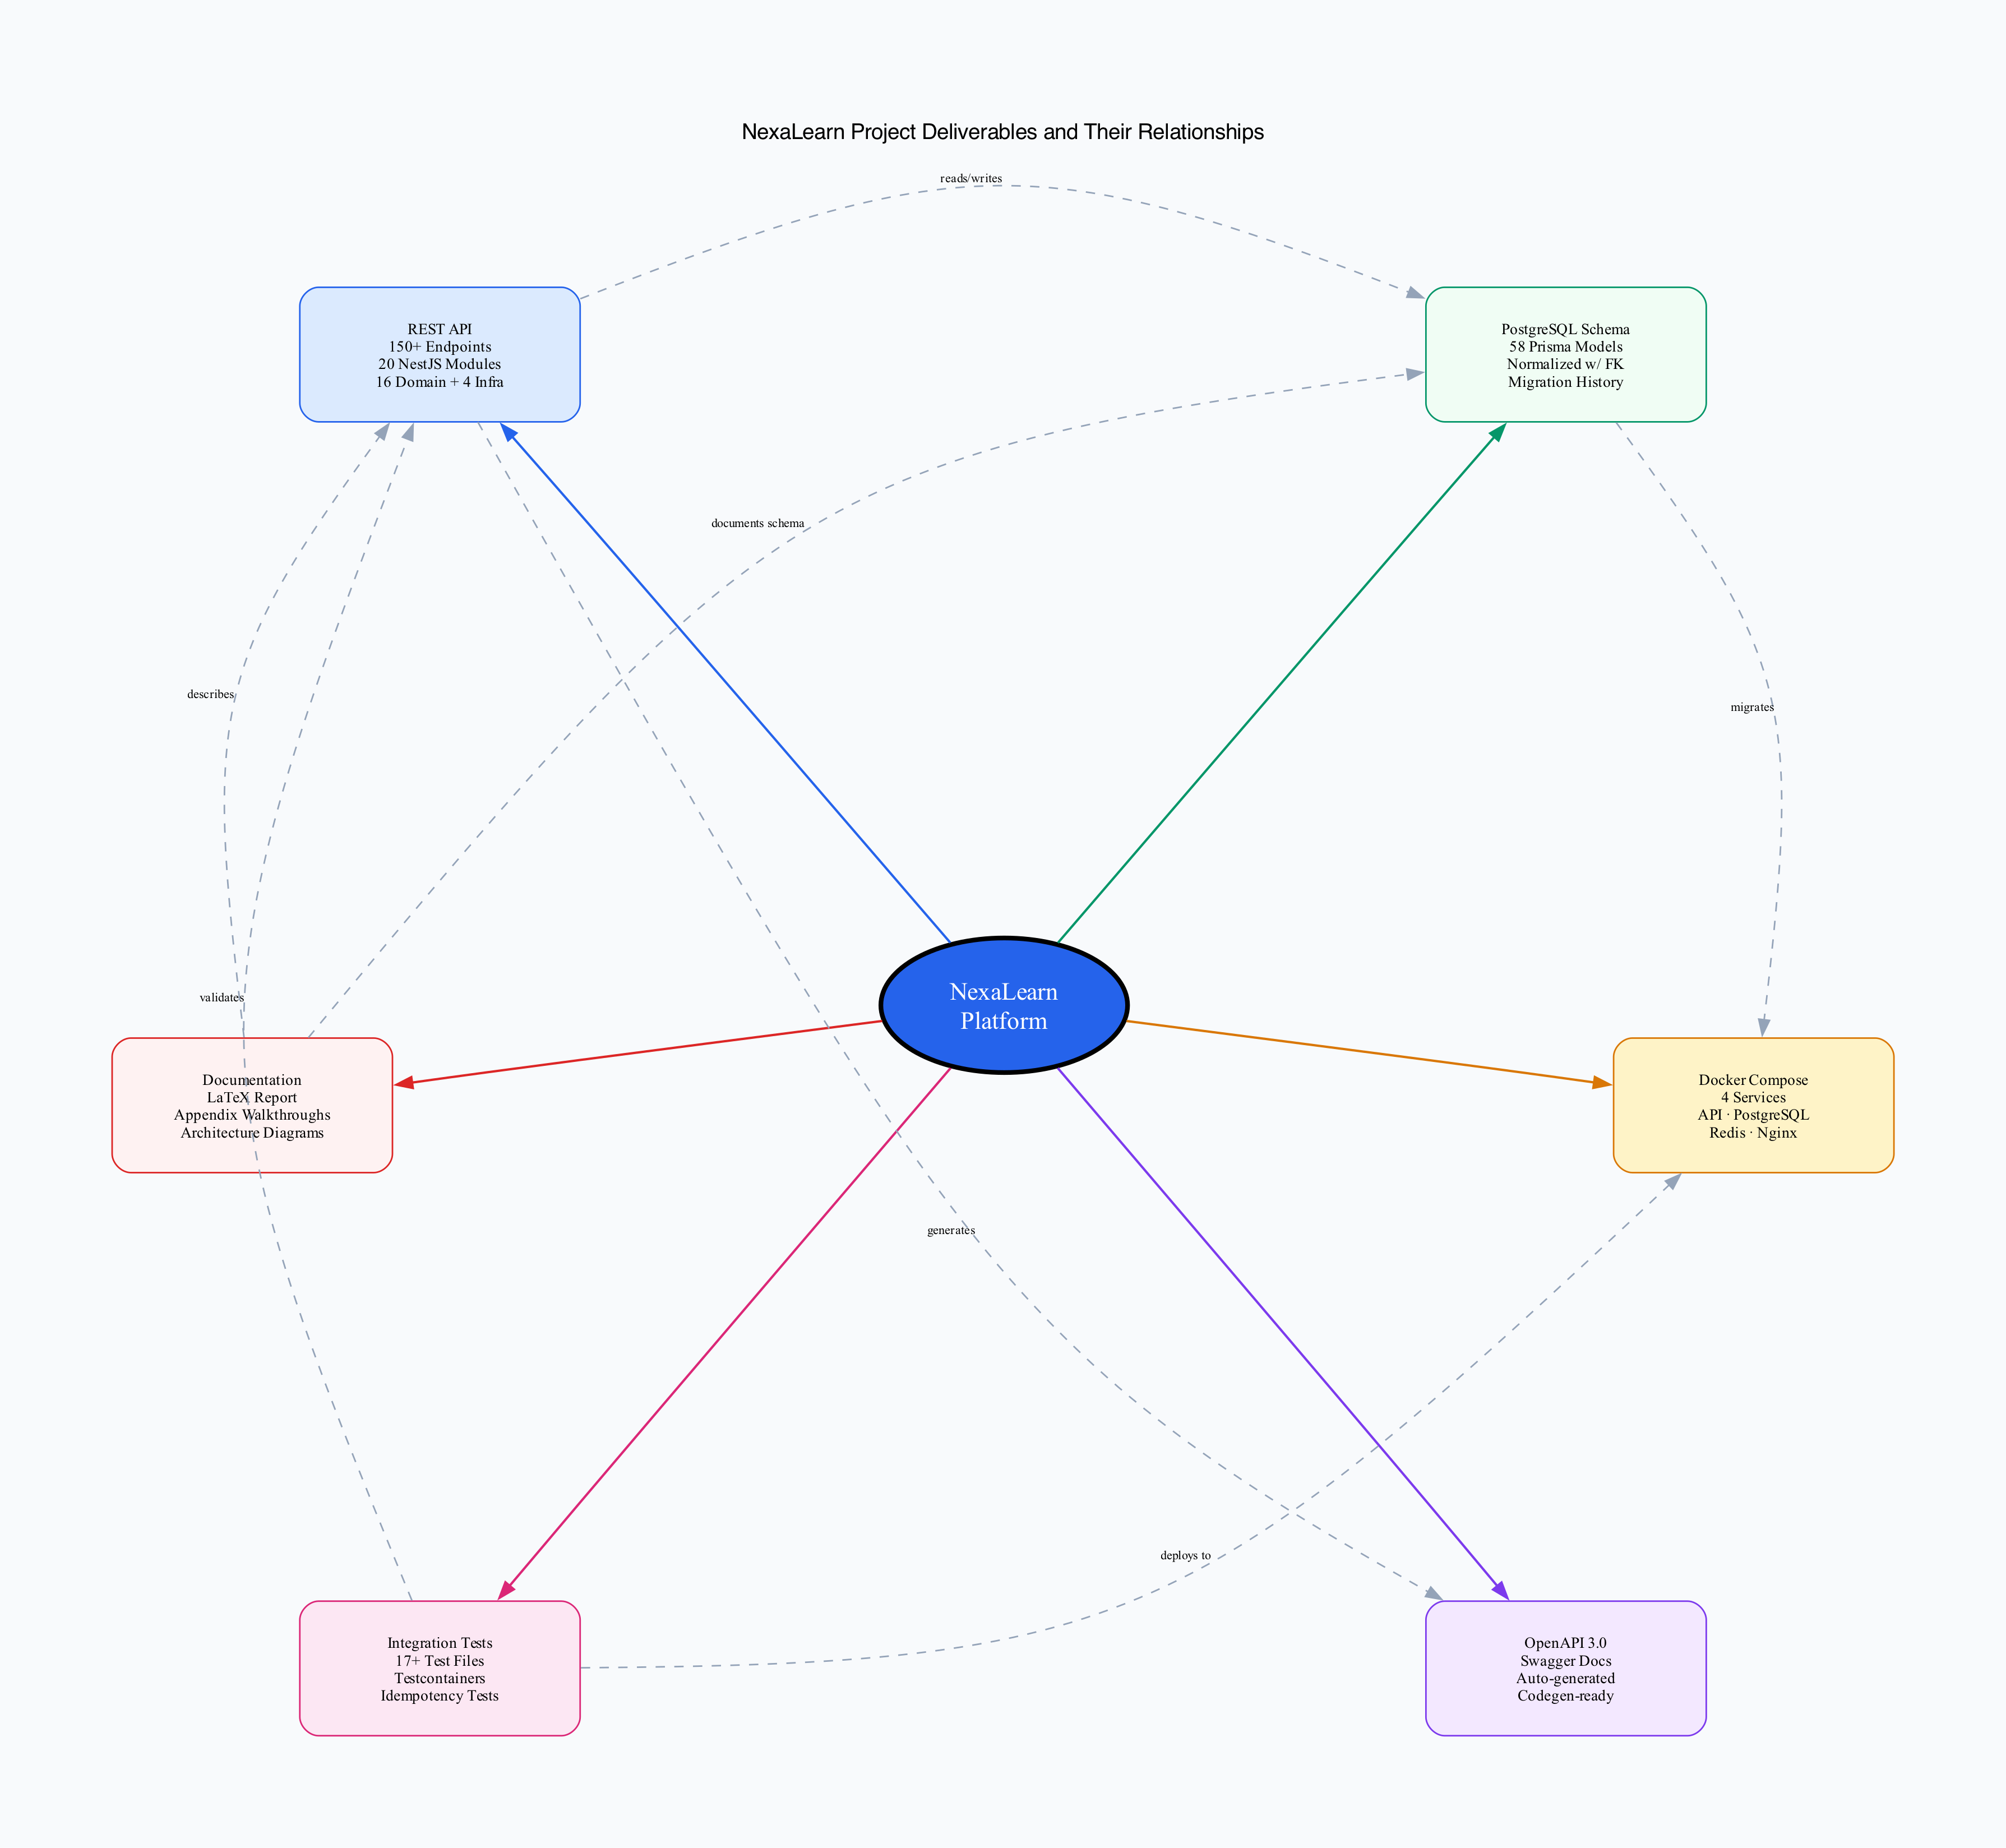
\includegraphics[width=0.90\textwidth]{images/deliverables_overview.png}
  \caption{Summary of NexaLearn Project Deliverables and Their Relationships}
  \label{fig:deliverables-overview}
\end{figure}

Figure~\ref{fig:deliverables-overview} illustrates dependencies among deliverables: the API implements business logic against the schema; migrations version the schema; Docker Compose deploys API and dependencies; OpenAPI documents the API surface; integration tests validate cross-module behaviour; and this report plus appendices capture design intent. Each outcome closes the loop between motivation (Section~\ref{sec:motivation}), problem definition (Section~\ref{subsec:problem-definition}), and objectives (Section~\ref{subsec:project-objectives}).

% =============================================================================
% Section 1.4: Document Organization
% =============================================================================

\section{Document Organization}
\label{sec:document-organization}

This report is structured to guide evaluators, future maintainers, and interested engineers from commercial and academic motivation through detailed engineering design, empirical verification, and critical reflection. Each chapter fulfils a distinct role in the narrative arc; together they satisfy the Cairo University Faculty of Engineering graduation project template while tailoring content to the NexaLearn backend domain. Table~\ref{tab:chapter-roadmap} provides a concise roadmap; subsections below expand the purpose and internal organisation of each chapter.

\begin{table}[H]
  \centering
  \caption{Roadmap of Report Chapters and Primary Focus Areas}
  \label{tab:chapter-roadmap}
  \small
  \begin{tabular}{@{}clp{7.8cm}@{}}
    \toprule
    \textbf{Ch.} & \textbf{Title} & \textbf{Primary Focus} \\
    \midrule
    1 & Introduction &
    Motivation, problems, objectives, outcomes, report structure \\
    2 & Market Visibility Study &
    Customers, competitors, business case, financial analysis \\
    3 & Literature Survey &
    DDD, Clean Architecture, technologies, prior work comparison \\
    4 & System Design and Architecture &
    Modules, diagrams, use cases, implementation patterns \\
    5 & System Testing and Verification &
    Test strategy, module/integration results, schedules \\
    6 & Conclusions and Future Work &
    Challenges, experience gained, limitations, extensions \\
    \midrule
    -- & References &
    Numbered citations in order of appearance \\
    A--E & Appendices &
    Tools, use cases, user guide, code docs, feasibility study \\
    \bottomrule
  \end{tabular}
\end{table}

\subsection{Chapter 2: Market Visibility Study}
\label{subsec:doc-ch2}

Chapter~2 positions NexaLearn within the commercial e-learning landscape. It opens with an introductory paragraph framing the market for backend platforms and independent course infrastructure. Section~2.1 identifies \textbf{target customers} in three segments: universities and educational institutions requiring data sovereignty and customisation; corporate learning and development (L\&D) departments needing SSO integration, compliance tracking, and ROI analytics; and independent course creators or edtech startups seeking white-label backends without revenue-sharing SaaS constraints.

Section~2.2 presents a \textbf{market survey} of competing platforms---Udemy for Business, Coursera, Teachable, Thinkific, Moodle, Open edX, and generic NestJS boilerplates---with dedicated subsections analysing strengths, weaknesses, architectural openness, and implications for NexaLearn differentiation. Section~2.3 develops the \textbf{business case and financial analysis}, estimating capital expenditure (development salaries, infrastructure setup), operational expenditure (cloud hosting, monitoring, support), projected sales volumes over five years, pricing strategy relative to competitors, monthly cash-flow projections, and the projected break-even date. This chapter demonstrates that NexaLearn is not only technically viable but commercially conceivable if productised.

\subsection{Chapter 3: Literature Survey}
\label{subsec:doc-ch3}

Chapter~3 supplies the theoretical and technological foundations required to understand design decisions in Chapters~4 and~5. An introductory paragraph outlines the chapter's two-part structure: engineering background, then comparative prior work.

Background sections (e.g., Sections~3.1--3.2) cover pivotal topics including \textbf{Domain-Driven Design} (entities, aggregates, bounded contexts, context maps), \textbf{Clean Architecture} and dependency inversion, \textbf{CQRS-lite} command/query separation, \textbf{event-driven architecture}, the \textbf{transactional outbox pattern}, and relevant platform technologies: NestJS module system, PostgreSQL ACID semantics, Prisma ORM, Redis caching patterns, Stripe payment lifecycles, Mux video pipelines, and AI speech/LLM integration patterns.

Section~3.3 presents a \textbf{comparative study of previous work}, reviewing recent academic publications and industry articles on e-learning platform architecture, microservice reliability, and LMS modernisation from approximately the past three years. Section~3.4 concludes with the \textbf{implemented approach}, justifying NexaLearn's modular monolith over premature microservice decomposition, and documenting adaptations (CQRS-lite rather than full event sourcing, outbox rather than Kafka in v1) appropriate to graduation project scope.

\subsection{Chapter 4: System Design and Architecture}
\label{subsec:doc-ch4}

Chapter~4 is the technical core, answering \textit{what was built} and \textit{how it was built}. It opens with assumptions (single-tenant deployment, English primary locale, external AI provider availability) and non-functional requirements (security, horizontal scalability of stateless API tier, observability via structured logging and audit trails).

Section~4.2 presents \textbf{system architecture} through block diagrams, deployment topology, and the three high-level module groupings:
\begin{itemize}
  \item \textbf{Learning Core} --- Auth, Courses, Enrollment, Media, Progress, Assessment, Certificates;
  \item \textbf{Engagement \& Commerce} --- Discussion, Reviews, Streak, Notifications, Payments, Search;
  \item \textbf{Platform \& Operations} --- Instructor Analytics, Admin, Audit, Events/Outbox, AI Pipeline, Prisma/Common infrastructure.
\end{itemize}

Subsequent sections (4.3 onward) decompose each major module following the faculty template substructure: \textit{functional description}, \textit{modular decomposition} (domain/application/infrastructure layers), \textit{design constraints}, and supplementary discussion with diagrams, sequence charts, ERD excerpts, and representative TypeScript code snippets. Event flows---enrollment activation, outbox processing, Mux webhook handling, AI callback ingestion---receive dedicated treatment because they embody cross-cutting reliability concerns introduced in Chapter~1.

\subsection{Chapter 5: System Testing and Verification}
\label{subsec:doc-ch5}

Chapter~5 documents verification strategy and results. Section~5.1 describes the \textbf{testing setup}: Docker Compose environments, Testcontainers PostgreSQL/Redis, mocked Stripe/Mux/AI providers where external calls are impractical in CI, and Jest as the test runner. Section~5.2 explains the \textbf{testing plan and strategy}, distinguishing unit tests (domain logic), integration tests (repository + outbox + webhook handlers against real database), and end-to-end HTTP tests (full request/response cycles).

Subsections~5.2.1 and~5.2.2 cover \textbf{module testing} and \textbf{integration testing} respectively, presenting representative test cases, expected versus actual outcomes, and defects discovered during development. Section~5.3 outlines the \textbf{testing schedule} aligned with development milestones. Section~5.4 provides \textbf{comparative results} where applicable---e.g., outbox throughput under concurrent workers, payment activation latency---in tabular or graphical form with interpretive commentary linking results back to Objective~8 (production-grade reliability).

\subsection{Chapter 6: Conclusions and Future Work}
\label{subsec:doc-ch6}

Chapter~6 synthesises the project narrative. Section~6.1 discusses \textbf{faced challenges}: Stripe webhook edge cases (delayed duplicates, metadata mismatches), coordinating Prisma migrations across team members, managing AI pipeline latency and cost, and balancing DDD purity with delivery deadlines. Section~6.2 reflects on \textbf{gained experience} in NestJS modular design, event-driven reliability, payment integration security, and technical writing.

Section~6.3 states \textbf{conclusions}: the extent to which objectives were met, distinctive features of NexaLearn (unified open reference, outbox-tested reliability, AI pipeline integration), and acknowledged limitations (single-region deployment, no bundled frontend in scope, dependence on external AI providers). Section~6.4 proposes \textbf{future work}: multi-tenant isolation, GraphQL adjunct APIs, recommendation engines, SCORM/xAPI import, localised content, Kubernetes deployment manifests, and third-party security audit.

\subsection{References and Appendices}
\label{subsec:doc-backmatter}

\textbf{References} follow Chapter~6, numbered in order of first citation throughout the report (faculty template style \texttt{[1], [2], \ldots}).

\textbf{Appendix~A} --- Development Platforms and Tools: hardware/software inventory, NestJS, Prisma, Docker, Stripe/Mux SDKs, AI tooling. \textbf{Appendix~B} --- Use Cases: formal use case diagrams and descriptions for student enrollment, instructor publishing, admin moderation. \textbf{Appendix~C} --- User Guide: step-by-step operational instructions for instructors and administrators with screenshots. \textbf{Appendix~D} --- Code Documentation: selected module walkthroughs and directory structure. \textbf{Appendix~E} --- Feasibility Study: expanded financial projections supporting Chapter~2.

\subsection{Reading Paths for Different Audiences}
\label{subsec:doc-reading-paths}

Readers may navigate selectively:
\begin{itemize}
  \item \textbf{Faculty evaluators} --- Chapter~1 (context), Chapter~4 (design depth), Chapter~5 (verification), Chapter~6 (reflection);
  \item \textbf{Future student maintainers} --- Chapter~4, Appendices~A and~D, plus repository README;
  \item \textbf{Industry reviewers} --- Chapter~1 objectives/outcomes, Chapter~3 patterns, Chapter~4 outbox/payment/AI sections;
  \item \textbf{Business stakeholders} --- Chapter~2 market study, Appendix~E feasibility.
\end{itemize}

This organisational structure ensures NexaLearn is documented as a complete, reproducible engineering contribution---not an isolated GitHub repository---and closes Chapter~1 by orienting the reader toward the detailed chapters that follow.

